
\documentclass[10pt]{article}

\usepackage{amsmath}
\usepackage{amssymb}
\usepackage{amsthm}
\usepackage[margin=0.75in]{geometry}
\setlength{\parindent}{0pt}
\usepackage{pgfplots}
\usepackage{mdframed}
\pgfplotsset{compat=1.18}
\usepackage[colorlinks]{hyperref}

\newtheorem{lema}{Lema}
\newmdtheoremenv{teorema}{Teorema}

\begin{document}

\section*{Ejercicio 1}

Defino dos eventos:

\begin{description}
    \item[A] ``Tatoh gana el torneo''

    \item[B]: ``Viper gana la primer partida y el torneo se decide en la quinta partida''
\end{description}

Quiero calcular:

\begin{align*}
    P(A|B)=\frac{P(A\cap B)}{P(B)}
\end{align*}

donde:

\begin{align*}
    P(A\cap B)&=P(\text{``Tatoh gana el torneo y Viper gana la primer partida y el torneo se decide en la quinta partida''})=\\
              &=P([V,V,T,T,T]\cup [V,T,V,T,T]\cup [V,T,T,V,T])\\
              &=0.6^3\times 0.4^2\times 3\\
    P(B)&=P(\text{``Viper gana la primer partida y el torneo se decide en la quinta partida''})=\\
        &P([V,V,T,T,T]\cup [V,T,V,T,T]\cup [V,T,T,V,T]\cup [T,T,V,V,V]\cup [T,V,T,V,V]\cup [T,V,V,T,V])\\
        &=0.6^3\times 0.4^2\times 3+0.6^2\times 0.4^3\times 3
\end{align*}

Entonces:

\begin{align*}
    P(A|B)=\frac{0.6^3\times 0.4^2\times 3}{0.6^3\times 0.4^2\times 3+0.6^2\times 0.4^3\times 3}=\frac{0.4}{0.6+0/4}=0.4
\end{align*}

\pagebreak

\section*{Ejercicio 2}

Defino dos variables aleatorias:

\begin{description}
    \item[A] $\sim U[2, 4]$
    \item[J] $\sim U[1, 3]$
\end{description}

Las función de densidad de probabilidad de $A$ y de $J$ son:

\begin{align*}
    f(a)&=\frac{1}{2},\quad a\in[2,4]\\
    f(j)&=\frac{1}{2},\quad j\in[1,3]
\end{align*}

y porque $A$ y $J$ son independientes:

\begin{align*}
    f(a, j)=f(a)f(j)=\frac{1}{4}\quad a\in[2,4], b\in[1,3]
\end{align*}

Quiero calcular:

\begin{align}
    P(J<A|A+J<5)=\frac{P(J<A\;\cap\;A+J<5)}{P(A+J<5)}
	\label{eq:targetProbEx2}
\end{align}

Puedo hacer esto gráficamente, dividiendo el área de la región gris en la Figure~\ref{fig:ex2} sobre el área debajo de la linea $A=5-J$, entre las lineas verticales y por encima de la linea horizontal $J=1$.

\begin{figure}
\centering
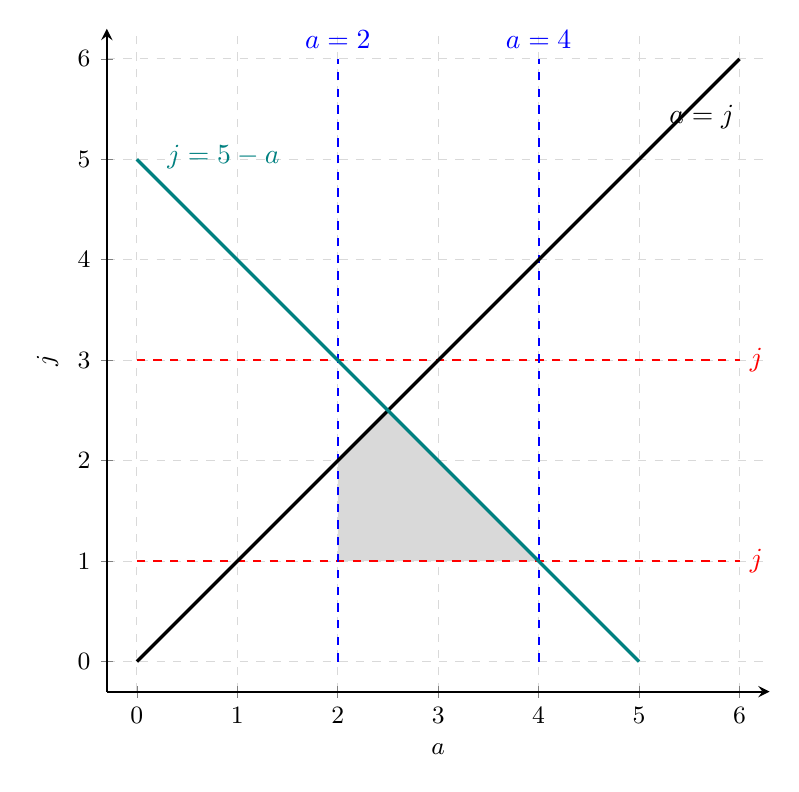
\begin{tikzpicture}
\begin{axis}[
    axis lines = left,
    xlabel = {$a$},
    ylabel = {$j$},
    xmin = 0, xmax = 6,
    ymin = 0, ymax = 6,
    xtick = {0,1,2,3,4,5,6},
    ytick = {0,1,2,3,4,5,6},
    grid = both,
    grid style = {dashed, gray!30},
    width = 10cm,
    height = 10cm,
    line width = 0.8pt,
    tick label style = {font=\small},
    label style = {font=\small},
    enlargelimits={abs=0.3}
]

% Shaded region satisfying all inequalities
\fill[gray!30] (axis cs:2,1) -- (axis cs:2,2) -- (axis cs:2.5,2.5) -- (axis cs:4,1) -- cycle;

% 3. Horizontal lines at j=1 and j=3
\addplot[red, thick, dashed, domain=0:6] {1};
\node[red, right] at (axis cs:6,1) {$j=1$};

\addplot[red, thick, dashed, domain=0:6] {3};
\node[red, right] at (axis cs:6,3) {$j=3$};

% 4. Vertical lines at a=2 and a=4
\draw[blue, thick, dashed] (axis cs:2,0) -- (axis cs:2,6);
\node[blue, above] at (axis cs:2,6) {$a=2$};

\draw[blue, thick, dashed] (axis cs:4,0) -- (axis cs:4,6);
\node[blue, above] at (axis cs:4,6) {$a=4$};

% 5. Diagonal line a=j
\addplot[black, very thick, domain=0:6] {x};
\node[black, above right] at (axis cs:5.2,5.2) {$a=j$};

% 6. Line j=5-a
\addplot[teal, very thick, domain=0:5] {5-x};
\node[teal, above right] at (axis cs:0.2,4.8) {$j=5-a$};

\end{axis}
\end{tikzpicture}

\caption{Necesito integrar la densidad sobre el área gris para calcular el numerador en Ec.~\ref{eq:targetProbEx2} e integrar la densidad debajo de la linea $J=5-A$, entre las lineas verticales y sobre la linea horizontal $J=1$, para calcular el denominador en la misma ecuación.}

\label{fig:ex2}

\end{figure}

También puedo calcular la probabilidad en Ec.~\ref{eq:targetProbEx2} analíticamente. Primero determino el punto en el eje $A$ en donde la diagonal $J=A$ se intersecta con la linea $J=5-A$. Si $J=A$ y $J=5-A$, entonces $A=2.5$.

\begin{align*}
	P(A<J\;\cap\;A+J<5)&=\int_2^{2.5}\int_1^af(a,j)\;djda+\int_{2.5}^4\int_1^{5-a}f(a,j)\;djda=\frac{1}{4}\left(\int_2^{2.5}\int_1^a\;djda+\int_{2.5}^4\int_1^{5-a}\;djda\right)\\
	                   &=\frac{1}{4}\left(\int_2^{2.5}(a-1)da+\int_{2.5}^4(4-a)da\right)=\frac{1}{4}\left(\left.(\frac{a^2}{2}-a)\right|_{a=2}^{2.5}+\left.(4a-\frac{a^2}{2})\right|_{a=2.5}^4\right)\\
					   &=\frac{1}{4}\left((0.625-0.0)+(8.0-6.875)\right)=\frac{1}{4}1.75\\
	P(A+J<5)&=\int_2^4\int_1^{5-a}f(a,j)\;djda=\int_2^4\int_1^{5-a}\frac{1}{4}\;djda=\frac{1}{4}\int_2^4\int_1^{5-a}\;djda=\frac{1}{4}\int_2^4(4-a)\;da\\
	        &=\frac{1}{4}\left.(4a-\frac{a^2}{2})\right|_{a=2}^4=\frac{1}{4}(8-6)=\frac{1}{4}2
\end{align*}

Entonces

\begin{align*}
    P(J<A|A+J<5)=\frac{P(J<A\;\cap\;A+J<5)}{P(A+J<5)}=\frac{1.75}{2}=0.875
\end{align*}

\pagebreak
\section*{Ejercicio 3}

Para calcular la varianza de $W$, voy a usar la expresión $Var(W)=E(W^2)-E^2(W)$.

\begin{align*}
    E(W)&=\int\int r i^2 f_{RI^2}(ri^2)\;dr\;di^2=\int\int r i^2 f_R(t)f_{I^2}(i^2)\;dr\;di^2=\left(\int rf_R(r)dr\right)\left(\int i^2f_{I^2}(i^2)di^2\right)\\
        &=E(R)E(I^2)\\
    E(W^2)&=\int\int r^2 (i^2)^2 f_{RI^2}(ri^2)\;dr\;di^2=\int\int r^2 (i^2)^2 f_R(t)f_{I^2}(i^2)\;dr\;di^2=\left(\int r^2f_R(r)dr\right)\left(\int (i^2)^2f_{I^2}(i^2)di^2\right)\\
        &=E(R^2)E((I^2)^2)
\end{align*}

para lo cual necesito obtener:

\begin{itemize}
    \item $E(R^2)$,
    \item $E(I^2)$, y
    \item $E((I^2)^2)$.
\end{itemize}

\begin{align*}
    E(R^2)=\text{Var}(R)+E^2(R)=2+100=102
\end{align*}

Definamos $Z=I^2$. Queremos calcular $E(Z)$ y $E(Z^2)$, para lo cual vamos a
obtener la función de densidad de probabilidad de $Z$.

\begin{align}
    F_Z(z)&=P(Z<z)=P(I^2<z)=P(I<\sqrt{z})=\frac{\sqrt{z}}{4},\quad\text{if}\;6\le\sqrt{z}\le
    10\;\text{or}\;36\le z\le 100\nonumber\\
    f_Z(z)&=\frac{\partial}{\partial z}F_Z(z)=\frac{1}{8}z^{-1/2}\nonumber\\
    E(Z)&=\int_{36}^{100}zf_Z(z)dz=\int_{36}^{100}z\frac{1}{8}z^{-1/2}dz=\frac{1}{8}\int_{36}^{100}z^{1/2}dz=\frac{1}{8}\frac{2}{3}\left.z^{3/2}\right|_{36}^{100}=\frac{1}{12}(10^3-216)=\frac{784}{12}\label{eq:EZ}\\
    E(Z^2)&=\int_{36}^{100}z^2f_Z(z)dz=\int_{36}^{100}z^2\frac{1}{8}z^{-1/2}dz=\frac{1}{8}\int_{36}^{100}z^{3/2}dz=\frac{1}{8}\frac{2}{5}\left.z^{5/2}\right|_{36}^{100}=\frac{1}{20}(10^5-6^5)=\frac{1}{20}92224\label{eq:EZ2}
\end{align}

Entonces

\begin{align*}
    E(W)&=E(R)E(Z)=10\;\frac{784}{12}=5\;\frac{392}{3}\\
    E(W^2)&=E(R^2)E(Z^2)=102\;\frac{1}{20}92224=51\;\frac{1}{10}92224=4703424.0=470342.4
\end{align*}

Finalmente

\begin{align}
    Var(W)=E(W^2)-E^2(W)=470342.4-25\;\frac{392^2}{9}=43497.96
    \label{eq:answerEx3}
\end{align}

Para verificar este calculo, simule 1000 muestras de W, calcule la
varianza de la muestra, y repetí este cálculo 1000 veces. De este modo obtuve 1000
valores de la varianza muestral. Cada valor de la varianza muestral es
diferente, pues las muestras son aleatorias. Si el valor de la varianza de $W$
obtenido analíticamente en Ec.~\ref{eq:answerEx3} es correcto, este valor
debería ser cercano a la media de las varianzas muestrales. Como muestra la
Figura~\ref{fig:ex3}, el valor de la media varianza muestral (linear vertical
discontinua) es cercano al valor de la varianza analítica (linea vertical
solida). El código Python que use para generar esta figura esta
\href{http://www.gatsby.ucl.ac.uk/~rapela/tmp/doEx3.py}{acá}.

\begin{figure}
    \centering
    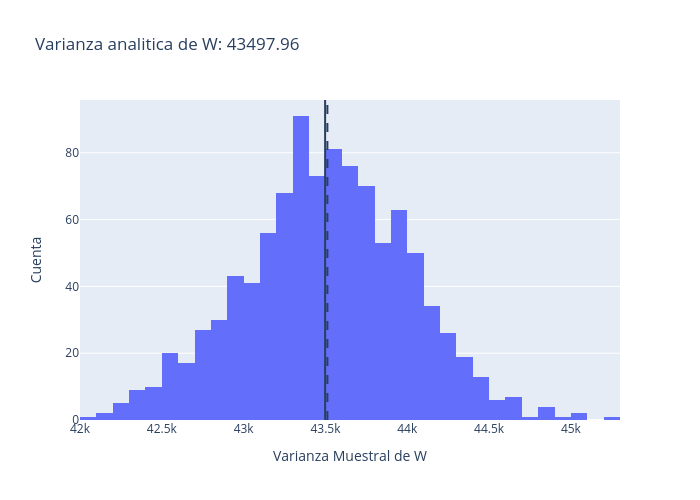
\includegraphics[width=6in]{../..//figures/fig_ex3.png}
    \caption{Histograma de varianzas muestrales. La media de las varianzas
    muestrales (linea vertical discontinua) es cercana a la varianza obtenida
    analíticamente en Ec.~\ref{eq:answerEx3} (linea vertical continua), lo que
    sugiere que la varianza analítica es correcta.}
    \label{fig:ex3}
\end{figure}

\pagebreak
\section*{Ejercicio 4}

Parafraseo la pregunta como ``Hallar la probabilidad de que el primer y el
tercer alumno lleguen con sandwiches de salchicha de burro dado que el segundo
alumno llego con un sándwich vegetariano.''

Asumo que la llegada de un alumno con su respectivo sándwich es independiente
de la llegada de previos y siguientes alumnos son sus respectivos sandwiches.

\begin{align*}
    P(1=S, 3=S | 2=V)=P(1=S|3=S, 2=V)P(3=S | 2=V)=P(1=S)P(3=S)=0.5^2=0.25
\end{align*}

\pagebreak
\section*{Ejercicio 5}

Asumo que los precios de las remodelaciones son independientes e idénticamente
distribuidos, con distribución normal con media 240 desvío estándar $\sigma$.
Es decir que para la i-esima remodelación, $R_i$, tenemos:

\begin{align*}
    R_i\sim\mathcal{N}(\mu=240, \sigma^2)
\end{align*}

Entonces, la distribución del promedio de 36 reformas va a ser una variable
aleatoria normal con media 240 y desvío estándar $\sigma/6$.
Es decir que para el promedio de 36 remodelaciones, $\bar{R}$, tenemos

\begin{align*}
    \bar{R}\sim\mathcal{N}(\mu=240, \sigma^2/36)
\end{align*}

Me interesa encontrar el valor de $\sigma$ para que:

\begin{align*}
    P(|\bar{R}-240|<0.5)=0.95
\end{align*}

o, lo que es lo mismo:

\begin{align*}
    P\left(\left|\frac{\bar{R}-240}{\sigma/6}\right|<\frac{0.5}{\sigma/6}\right)=0.95
\end{align*}

Pero sabemos que $Z=\frac{\bar{R}-240}{\sigma/6}$ es una variable aleatoria normal
estándar, por lo que $\frac{0.5}{\sigma/6}$ debe ser el valor $z$ que deja
un total de 0.025 de probabilidad a la derecha. Es decir que
$\frac{0.5}{\sigma/6}$ debe ser el 97.5 percentil de la distribución normal
estándar, cuyo valor es $z_{0.975}=1.96$.

\begin{align*}
    \frac{0.5}{\sigma/6}=z_{0.975}=1.96
\end{align*}

Entonces

\begin{align*}
    \sigma=\frac{0.5\times 6}{1.96}=\frac{3}{1.96}=1.53
\end{align*}

\pagebreak
\section*{Apéndice al ejercicio 3}

Delfi se ahorró el cálculo de $f_Z(z)$ para obtener $E(Z)$. Calculo $E(Z)$
como sigue:

\begin{align*}
    E(Z)=E(I^2)=\int_6^{10}i^2f_Y(y)dy=\frac{1}{4}\int_6^{10}i^2dy=\frac{1}{4}\left.\frac{i^3}{3}\right|_{i=6}^{10}=\frac{1}{12}\left(10^3-6^3\right)=\frac{784}{12}
\end{align*}

obteniendo el mismo resultado que en la Ec.~\ref{eq:EZ}.
%
También se ahorró el cálculo de $f_Z(z)$ para obtener $E(Z^2)$:

\begin{align*}
    E(Z^2)=E(I^4)=\int_6^{10}i^4f_Y(y)dy=\frac{1}{4}\int_6^{10}i^4dy=\frac{1}{4}\left.\frac{i^5}{5}\right|_{i=6}^{10}=\frac{1}{20}\left(10^5-6^5\right)
\end{align*}

obteniendo el mismo resultado que en la Ec.~\ref{eq:EZ2}.

¿Porque funciona le método de Delfi? El siguiente lema lo demuestra.
\textbf{Este lema es muy importante, pues prueba que para calcular el valor
esperado de una función de una variable aleatoria no hace falta calcular la
función de densidad de probabilidad de la variable aleatoria transformada.}

\begin{lema}

    Si $X$ es una variable aleatoria en $\mathbb{R}$, con función de densidad
    de probabilidad $f_X(x)$, con soporte en $[a, b]$, y $g:[a,
    b]\rightarrow I$ es una función monotónica no decreciente (i.e.,
    $y_1\le y_2$ implica que $g(y_1)\le g(y_2)$), donde $I\in\mathbb{R}$ es un
    intervalo, entonces

\begin{align*}
    E(g(X))=\int_a^bg(x)f_X(x)dx
\end{align*}

\end{lema}

\begin{proof}

    Definimos la variable aleatoria $Y=g(X)$. Como $X\in[a,b]$, y porque $g$ es
    monótona no decreciente, se cumple que $Y=g(X)\in[g(a),g(b)]$.

    Quiero calcular $E(g(X))=E(Y)$
    para lo cual voy a derivar la función de densidad de probabilidad de $Y$,
    $f_Y(y)$. Empiezo calculando la función de distribución acumulada,
    $F_Y(y)$.

    \begin{align*}
        F_Y(y)=P(Y<y)=P(g(X)<y)=P(X<g^{-1}(y))=F_X(g^{-1}(y))
    \end{align*}

    done $g^{-1}$ existe, pues $g$ es monotónica, y obtengo $f_Y(y)$ derivando
    $F_Y(y)$.

    \begin{align}
        f_Y(y)=F'_Y(y)=F'_X(g^{-1}(y))\;(g^{-1})'(y)=f_X(g^{-1}(y))\;(g^{-1})'(y)=\frac{f_X(g^{-1}(y))}{g'(g^{-1}(y))}\label{eq:f_Y}
    \end{align}

    En la segunda igualdad de la Ec.~\ref{eq:f_Y} usamos la regla de la cadena
    de la derivada, y en la última igualdad usamos el resultado
    $(g^{-1})'(y)=1/g'(g^{-1}(y))$\footnote{$g\left(g^{-1}(y)\right)=y$,
    derivando ambos lados de la igualdad, usando la regla de la cadena de la
    derivada, $g'\left(g^{-1}(y)\right)\;(g^{-1})'(y)=1$, por lo que sigue que
    $(g^{-1})'(y)=1/g'\left(g^{-1}(y)\right)$}.  Entonces

    \begin{align*}
        E(g(X))=E(Y)=\int_{g(a)}^{g(b)}yf_Y(y)dy=\int_{g(a)}^{g(b)}y\frac{f_X(g^{-1}(y))}{g'(g^{-1}(y))}dy\label{eq:EgX}
    \end{align*}

    Ahora vamos a utilizar el
    \href{https://es.wikipedia.org/wiki/Sustituci%C3%B3n_en_integraci%C3%B3n#Integrales_definidas}{teorema
    del cambio de variables} que dice:

    \begin{teorema}[Cambio de variables]

        Dada una función $\varphi:[a,b]\rightarrow I$ continuamente
        diferenciable, donde $I\in\mathbb{R}$ es un intervalo, y una función
        continua $f: I\rightarrow\mathbb{R}$, entonces

        \begin{align*}
            \int_a^bf(\varphi(x))\varphi'(x)dx=\int_{\varphi(a)}^{\varphi(b)}f(u)du
        \end{align*}
    \end{teorema}

    Aplicando este teorema con $\varphi(x)=g(x)$ y
    $f(y)=y\frac{f_X(g^{-1}(y))}{g'(g^{-1}(y))}$ obtenemos lo que queríamos
    probar.

    \begin{align*}
        E(g(X))=\int_{g(a)}^{g(b)}y\frac{f_X(g^{-1}(y))}{g'(g^{-1}(y))}dy=\int_a^bg(x)\frac{f_X(g^{-1}(g(x))))}{g'(g^{-1}(g(x)))}g'(x)dx=\int_a^bg(x)\frac{f_X(x)}{g'(x)}g'(x)dx=\int_a^bg(x)f_X(x)dx
    \end{align*}

\end{proof}
\end{document}
